% SEN421 Fall 2026 -- Topic 2 (Part A): Virtual Machines vs. Containers
% Built on the official course template (IEEEtran, conference, A4).

\documentclass[conference,a4paper]{IEEEtran}

\usepackage{amsmath,amssymb,amsfonts}
\usepackage{graphicx}
\usepackage{textcomp}
\usepackage{xcolor}
\usepackage{booktabs}
\usepackage{array}
\usepackage{listings}
\usepackage{url}
\usepackage{xurl} % lets long URLs (e.g. the pricing calculator link) break at any character
\usepackage{hyperref}
\usepackage{cite}
\usepackage{pgfplots}
\usepackage{pgfplotstable}
\pgfplotsset{compat=1.17}

\lstset{
	basicstyle=\ttfamily\footnotesize,
	keywordstyle=\color{blue}\bfseries,
	commentstyle=\color{gray}\itshape,
	stringstyle=\color{red},
	numbers=left,
	numberstyle=\tiny\color{gray},
	numbersep=5pt,
	frame=single,
	breaklines=true,
	captionpos=b,
	tabsize=4
}

\newcommand{\todo}[1]{\textcolor{red}{[TODO: #1]}}

\begin{document}

\title{Virtual Machine or Container? Measuring Startup Time, Footprint, and Throughput of a Supply Chain API\\
	{\footnotesize SEN421 --- Cloud Architecture and Services, Course Project, Fall 2026\\
		Istanbul Ayd\i n University}
}

\author{\IEEEauthorblockN{G\"ozde G\"on\"ul}
	\IEEEauthorblockA{\textit{Department of Computer Engineering}\\
		\textit{Istanbul Ayd\i n University}\\
		Istanbul, Turkey \\
		Student ID: B2205.010143 \\
		gozdegonul@stu.aydin.edu.tr}
}

\maketitle

\begin{abstract}
When the load of an application in the cloud environment increases, new copies must be created and these copies must be started quickly to balance the load. The speed parameter involved in this process varies depending on the choice of virtual machine and container. This study measures the speed difference with the same application in part A of issue 2 and calculates costs with autoscaling. This study includes a Supply Chain web API with medium complexity. The Supply Chain Web API was run to compare the Ubuntu virtual machine and Docker Container on VirtualBox, which has two processor cores and two gigabytes of memory. The comparison was repeated three times for 50 simulated users in both cases, and the results were recorded. The results included initial request response time, applications using space, and memory usage comparisons. As a result of the measurements, containers respond to the first request within an average of 0.5 seconds, while for VirtualBoxes this time was approximately 71 seconds. Containers also used 228 megabytes of disk space instead of 6 gigabytes and responded to about six times more requests. The study included Amazon Web Services (AWS) pricing alongside the test results. In the calculations, the monthly fees for virtual machines were measured at \$37, while the monthly fees for containers were measured at \$83. As a result, containers are suitable for faster workloads, while virtual machines are more commonly used for fixed workloads.
\end{abstract}

\begin{IEEEkeywords}
cloud computing, virtualization, containers, Docker, performance evaluation
\end{IEEEkeywords}

% ---------------------------------------------------------------------------
\section{Introduction}
\label{sec:introduction}

As the states requested by users change in cloud computing, resources can be quickly added and freed, which actually promises rapid flexibility~\cite{b1}. A real-life example of the platform launching new copies created when the number of users increases and distributing requests among these copies can be given as a real-life example. The speed at which new copies are created is proportional to users' wait times. Longer creation time causes the workload to be distributed among existing copies and causes users to wait longer for responses.

Virtual machines and containers are the two most commonly used ways to package an application in the cloud. Virtual machines run their operating systems by the hypervisor, while containers share the main system kernel to package the application and the libraries required for the application~\cite{b5}. Previous studies have shown that most virtual machines and containers perform the same or perform better in tests~\cite{b6,b7}. Many small-scale companies and developers use Windows laptops to test their systems. In this case, Docker running on a lightweight virtual machine shares the hypervisors and processor on the desktop with Hyper-V. In these cases, differences between environments cannot be clearly measured.

This study was conducted to answer the question included in ``Topic 2, Part A.'' The question within this scope aims to find the difference between the same web application and the virtual machine in terms of startup time, disk and memory usage, response time, and number of processed requests. The topic also performs cost scaling using autoscaling. This study sought answers to these questions using the Supply Chain Web API prepared on Node.js and a Windows-based laptop. The virtual machines used in the study were set up via the Ubuntu Server virtual machine, and both the container and virtual machines have two processor cores and 2 gigabytes of memory. Tests were repeated three times for both the virtual machine and the container, and the results were recorded. As a result of the tests, cost measurements were made. Costs were calculated using the AWS Pricing Calculator.

This section explains the introduction of the article. In the following sections of the article, the concepts of virtual machines and containers are angled, and the studies are examined. The architecture of the study was derived, and measurements were made to make comparisons.

% ---------------------------------------------------------------------------
\section{Background and Related Work}
\label{sec:related_work}

This study was created using two different alternatives. Comparisons were made to determine which isolated the application better and which environments the application needed to function, and the topic was reinforced with resource scanning. In this section, the definitions of Virtual Machines and Containers were primarily determined, and their flexibility and startup times were compared.

\subsection{Virtual Machines}
Virtualization allows a physical computer to be divided into several virtual machines with their own operating systems. In the hardware section, real memory, disks, and CPU are shared from the physical machine to each virtual machine~\cite{b2}. Hypervisors are divided into two groups according to their areas of use.
\begin{itemize}
	\item \textbf{Type 1 Hypervisor:} This hardware-based hypervisor is mostly preferred by cloud providers~\cite{b2}.
	\item \textbf{Type 2 Hypervisor:} this hypervisor is used as an application for operating systems located on hosts~\cite{b2}.
\end{itemize}
This study was conducted with a Type 2 Hypervisor.

NAT gates perform network address translation. This process is done by hiding the virtual machine behind the host and forwarding the selected computer's ports~\cite{b4}. Because they contain an operating system, virtual machines have strong isolation and require disk space measurable in gigabytes and use memory even when not in use. In addition, the operating system must boot before applications can be started.

\subsection{Containers}
Containers are packages that contain everything necessary for an application along with their libraries. The biggest difference compared to virtual machines is that they share the kernel of the operating system~\cite{b5}. The Linux kernel provides containers with process, file, and network interfaces, isolating namespaces that give this appearance and limiting resources according to control groups~\cite{b3}. These limits are used in Docker to determine the number of processors and maximum memory~\cite{b3}. Therefore, when Docker starts, processes start instead of the operating system. Containers require the Linux kernel to run, and this operation was carried out on a Windows-based laptop and ran within a Linux virtual machine based on Linux Subsystems (WSL~2) for Windows Docker Desktop startup operations.

\subsection{Flexibility and Startup Time}
The NIST definition, which lists fast flexibility, one of the core features of cloud computing, scales capabilities according to demand and, in some cases, enables automatic provisioning and release~\cite{b1}. In autoscaling, threshold values are checked. If any criterion exceeds this value, new instances are added for that criterion~\cite{b2}. The proper functioning of the system depends on the response times of these created instances to requests. Therefore, startup time is considered the main criterion in this study.

\subsection{Related Studies}
When a literature review is conducted, two studies that most closely resemble this study stand out.
\begin{itemize}
	\item \textbf{Felter et al.~\cite{b6}:} In this study, a Docker container and a KVM virtual machine were compared on a server. As a result of the comparison, it was determined that most containers gave the same results or performed better than virtual machines in most tests. Additionally, overhead was observed in virtual machines, and this formation was mostly observed in input/output (I/O) operations. On the Docker side, NAT gates were observed to cause additional workload in the network part.
	\item \textbf{Morabito et al.~\cite{b7}:} This study compared two different virtualization methods. The compared methods are hypervisor-based virtualization and light virtualization. The report stated that containers were closer to local performance in terms of performance, while hypervisors created additional load.
\end{itemize}
In both studies reviewed in the literature, a Type 1 hypervisor was used. In this study, a Windows-based laptop activated by Hyper-V, which is generally used for small teams and students, is used. Type 2 is used as the hypervisor and evaluations are conducted with Docker Desktop. Cost, resource usage, and startup times were also included in this study.

% ---------------------------------------------------------------------------
\section{System Design}
\label{sec:design}

This part of the study includes the system's design and comparison setup. The architecture of the test environment, the applications used, and alternative comparisons are discussed. Elements outside the platform are kept the same in the design, and differences in measurement results are attributed to the choice of virtual machine and container.

\subsection{Architecture}
This study used a Windows 11-based laptop with an Intel Core i5-12450H processor and 16\,GB of memory enabled in both virtual machines and containers. The overall architectural structure of the study is shown in Fig.~\ref{fig:architecture}.

\begin{figure*}[t]
	\centering
	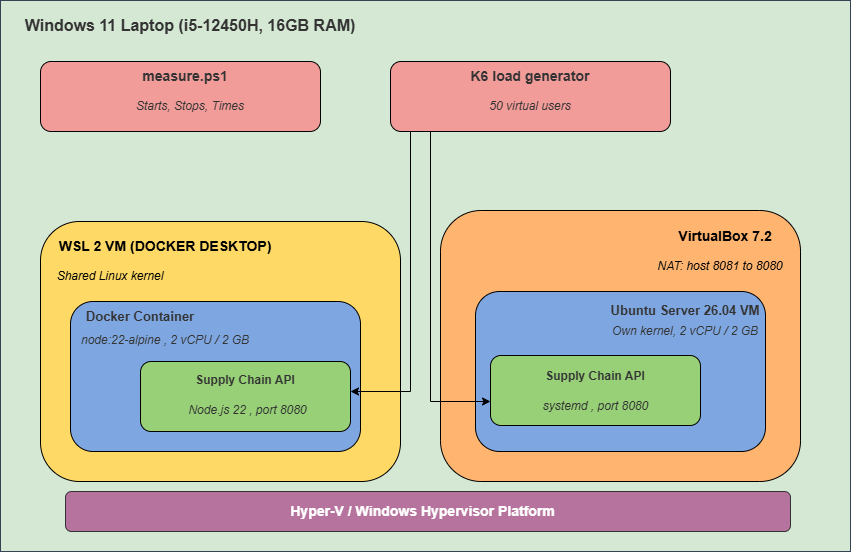
\includegraphics[width=0.85\textwidth]{architecture.png}
	\caption{Overall architecture of the test setup. The same supply chain API runs in a Docker container inside Docker Desktop's WSL~2 virtual machine (left) and in an Ubuntu virtual machine on VirtualBox (right), both on top of Hyper-V. k6 on the same laptop sends the HTTP load; measure.ps1 starts, stops and times both alternatives.}
	\label{fig:architecture}
\end{figure*}

As seen in Fig.~\ref{fig:architecture}, the operation consists of two main parts. In the structure shown on the left, Docker Desktop runs the container on the WSL~2 VM. After this run, the container is made accessible on port 8080 on the host. In the structure on the right side, VirtualBox runs an Ubuntu Server virtual machine via the Windows Hypervisor Platform, redirecting port 8081 to port 8080 on the virtual machine, and port 2222 on the host to the virtual machine's SSH port via the NAT port. K6 is used to generate payload~\cite{b8}. The ``measure.ps1'' script run on the host starts and stops virtual machines and containers, waits for the application to respond via the ``health'' endpoint, then performs load tests and saves the measurements to a CSV file. Initiates alternatives sequentially to avoid processor and memory competition.

\subsection{Application}
In this study, a supply chain Rest API consisting of a Node.js file was used. This API does not require an additional package and can therefore be used on both virtual machines and containers. This API stores all data in memory and generates the data randomly using a fixed value (seed). Therefore, in both distribution models, it provides services with data on the same 20 warehouses, 50 suppliers, 500 products with a 90-day sales history, and 250 products stocked in each warehouse. There are 22 endpoints within the Rest API. The 22 endpoints within the API; provide listing, querying processes, order creation, and order status tracking. Additionally, it uses the Dijkstra algorithm to find the shortest land route between the two warehouses. The ``Forecast'' endpoint within the API uses Holt's linear exponential smoothing method to forecast demand for a product; It uses a grid search method of $49 \times 49$ values to determine two parameters.

Another endpoint within the API is ``Replenishment.'' This API calculates the economic order quantity, safety stock, and reorder point for each product in the warehouse. The ``/health'' endpoint; provides the host name, uptime, and memory usage reporting, while the measurement script uses this endpoint to decide whether the application is ready.

\subsection{Compared Alternatives}
The application works with different applications tools in the virtual machine and container.
\begin{itemize}
	\item \textbf{Virtual Machine:} The application runs on virtual machines running Node.js 22 on Ubuntu Server 26.04.1 LTS. The user account used for tests is unprivileged and configured with the ``systemd'' service. The virtual machine used has 2048\,MB of memory and a dynamically allocated 20\,GB disk. Automatic updates are disabled for the guest operating system to prevent system shutdown delays.
	\item \textbf{Container:} The application runs on an image created based on ``node:22-alpine'' in containers. The image run on it runs as an unprivileged account named ``node'' and contains only the application file. The container is started with the ``\texttt{-{}-cpus 2}'' and ``\texttt{-{}-memory 2g}'' options; the goal here is for both virtual machines and containers to have the same number of memory and processors~\cite{b3}.
\end{itemize}
Both alternatives use the same application and Node.js version. The aim of this study is not to compare the difference between the application but the difference in the platform.

\subsection{Requirements and Responsibilities}
For the application to work on both virtual machines and containers, environments must provide the same API and data, run users without privileges, be accessible from the host via a fixed port, report availability via the ``health'' endpoint, and perform startup and stop via a script without manual intervention. However, the tasks that both must undertake in the maintenance part of virtual machines and containers vary. Tracking security updates for virtual machines is very important. Additionally, the task team is responsible for the entire guest operating system, including Node.js installation and service configuration. Image maintenance for the container is very important, and by updating the operating system layer, the task team reconstructs the image from a newer base image. In the cloud environment, the task team applies patches to the customer guest operating system in Amazon EC2. In AWS Fargate, the service provider manages the servers running the containers. This difference in responsibilities is addressed in Section~\ref{sec:discussion} along with the cost factor.

% ---------------------------------------------------------------------------
\section{Methodology}
\label{sec:methodology}

The measurements included in this study were not done manually. The measurements were designed through scripted runs designed to answer the research question. This section explains the methods used to predict the test environment, metrics, load testing, measurement procedure, and cloud cost under the headings.

\subsection{Test Environment}
All measurements included and reported in the study were performed on laptops with Windows 11 infrastructure and connected to electricity, as defined in Section~\ref{sec:design}. The software versions used in the study are detailed in Table~\ref{tab:environment}.

\begin{table}[htbp]
	\caption{Experimental Environment}
	\label{tab:environment}
	\centering
	\footnotesize
	\begin{tabular}{|l|p{0.58\columnwidth}|}
		\hline
		\textbf{Property} & \textbf{Value} \\
		\hline
		Host & Intel Core i5-12450H, 16\,GB RAM, Windows 11 Home 25H2 (build 26200), Hyper-V enabled \\
		\hline
		VM platform & VirtualBox 7.2.22, Ubuntu Server 26.04.1 LTS, 20\,GB VDI \\
		\hline
		Container platform & Docker Desktop, Docker Engine 29.9.3 (WSL 2 backend), image \texttt{node:22-alpine} \\
		\hline
		Limits (both) & 2 vCPU, 2\,GB memory \\
		\hline
		Application & Supply chain REST API, Node.js 22, 22 endpoints, no external libraries, synthetic data \\
		\hline
		Load test tool & k6 v2.4.0, 50 virtual users, no think time \\
		\hline
		Test duration & 2 minutes per run, 60\,s cooldown \\
		\hline
		Repetitions & 3 per alternative \\
		\hline
	\end{tabular}
\end{table}

On the computer where the work was done, since Hyper-V was enabled, the VirtualBox virtual machine ran on the Windows Hypervisor Platform instead of its own core drive. The tested system and the load generator were run on the same laptop. As a result, network activities between the machines were eliminated. This caused the k6 and the application to share the same processor.

\subsection{Metrics}
Time measurements were made within the application included in the study. The first of these measurements was startup time. In addition to this measurement, a query was performed every 50\,ms to measure the time from the moment the start command was given until the `/health' endpoint returns a successful response. For both alternatives, the ``Cold start'' and ``Warm start'' scenarios were used in the measurements. For cold startup, virtual machines were shut down, containers were rebuilt and started from the image. For hot startup, the virtual machine resumed from a saved state, while the stopped container was restarted. After the startup time measurements were completed, stop time measurements began. These measurements measured the time elapsed from the time the stop request was sent until the platform notified the completion of the stopping operation. The stop process has different meanings for the two alternatives included in the study. Virtual machines run the ACPI shutdown command to perform the stopping operation, while containers run the `docker stop' command. The size of the virtual disk file and the image size in the containers represent the disk footprint of the disks. Memory usage was also tested in the measurements and examined at three levels.
\begin{itemize}
	\item \textbf{Application:} First, the application's own memory usage was measured. This measurement value is actually sent by the `/health' endpoint, and the sent value is the ``resident set size'' (the set size built into memory).
	\item \textbf{Platform:} Secondly, Platform memory usage was measured. In these measurements, virtual machines and containers were examined. The memory usage of virtual machines is given by the ``working set'' value of the VirtualBox process located on the host computer. The container receives memory usage at the value reported by Docker~\cite{b3}. Since the containers in the study run within their own WSL~2 virtual machine, the memory usage of the respective virtual machine and containers was also tested and reported.
	\item \textbf{Performance:} Thirdly, a performance measurement was provided. Performance was defined by response time obtained from the K6 load generator summary included in the study, the number of requests processed per second (throughput), and the rate of failed requests~\cite{b8}.
\end{itemize}

\subsection{Load Test}
The load test included in the study was conducted with 50 virtual users for two minutes using the k6 tool. Since refreshes were performed without waiting time, the application was continuously run at full capacity. The purpose of each iteration is to simulate a short user session. In this simulation, products were listed in order, stock status of a product was checked, a page from the warehouse inventory was performed, an order was created for two products, demand estimation was requested, and route determination was carried out between the two warehouses. Additionally, a replenishment plan was requested for 10\% of the iterations. Not every requested stock may be available. In these cases, the order is rejected with the HTTP 409 status code. Since this is a natural flow of the system, it is not considered an error.

\subsection{Procedure}
The PowerShell script included in this study performed the necessary steps for both virtual machines and containers in the same order and automatically. Fixed specific tasks were included in the execution processes. These tasks were handled in order: cold startup, 30-second idle (memory usage was measured), two-minute load test (memory measurement was performed mid-test), stop, and finally hot startup and stop steps. Cooldown times were added between the measurements, leaving the duration at 60 seconds. Tests for both alternatives were repeated three times each, and the results, mean values, and sample standard deviations were calculated and recorded. Measurements were performed sequentially, and no simultaneous measurements were performed. First, tests were performed for the container, then for the virtual machine. At the start of the tests, automatic updates were enabled but were later disabled because it was detected to delay shutdown time. Although the virtual machine was started several times during the tests, traffic flow could not be provided over NAT port forwarding. To resolve this, the script shut down and restart the virtual machine. In the results section, only successful startups were recorded. Logs of such events are included in the measurement report in the project repo on GitHub.

\subsection{Cost Estimate}
Estimated Cloud costs were derived as a result of the study. For these estimated estimates, the AWS Pricing Calculator was used~\cite{b9}. The calculator used the Europe (Frankfurt) region and the ``on-demand'' pricing model as regions. For the virtual machine, the Amazon EC2 t3.medium instance and for the container calculation was performed using the AWS Fargate task. For both alternative models, normally two virtual processors and 2\,GB of memory were used. However, since the calculation via Fargate was not available, calculations were made using 4\,GB of memory. Pricing scenarios are two: a service running all month (730 hours) and a service running for half the duration (365 hours). The calculations assumed that data transfer did not exceed the monthly free usage quota provided by Amazon~\cite{b10}.

% ---------------------------------------------------------------------------
\section{Results}
\label{sec:results}

This section of the study contains the measurements obtained from the tests performed. The average of tests performed three times for each of the two alternatives and the sample standard deviation are summarized in Table~\ref{tab:results}.

% Generated by scripts/summarize.js -- do not edit by hand
\begin{table}[htbp]
\caption{Measured Results (Mean $\pm$ Standard Deviation, 3 Runs)}
\label{tab:results}
\centering
\footnotesize
\resizebox{\columnwidth}{!}{%
\begin{tabular}{|l|c|c|c|}
\hline
\textbf{Metric} & \textbf{Unit} & \textbf{VM} & \textbf{Container} \\
\hline
Disk footprint & MB & 6138 & 228 \\
\hline
Start time (cold) & ms & 70736 $\pm$ 5081 & 552 $\pm$ 285 \\
\hline
Start time (warm / resume) & ms & 15387 $\pm$ 1459 & 320 $\pm$ 26.5 \\
\hline
Stop time & ms & 10184 $\pm$ 1134 & 432 $\pm$ 28.8 \\
\hline
App process memory, idle & MB & 58.1 $\pm$ 0.1 & 60.8 $\pm$ 0.3 \\
\hline
Platform memory, idle & MB & 844 $\pm$ 16.9 & 12.4 $\pm$ 0.9 \\
\hline
Platform memory, under load & MB & 858 $\pm$ 15.3 & 58.4 $\pm$ 1.8 \\
\hline
Docker backend VM memory, idle & MB & -- & 1290 $\pm$ 160 \\
\hline
Response time, median & ms & 176 $\pm$ 87.9 & 21.3 $\pm$ 0.6 \\
\hline
Response time, p95 & ms & 253 $\pm$ 104 & 39.6 $\pm$ 1.3 \\
\hline
Throughput & req/s & 368 $\pm$ 223 & 2174 $\pm$ 66.0 \\
\hline
Failed requests & \% & 0.03 $\pm$ 0.03 & 0.00 $\pm$ 0.00 \\
\hline
\end{tabular}}
\end{table}


The rest of this section explains startup and shutdown processes, resource usage, performance under load, and estimated cloud cost calculations with graphs and tables.

\subsection{Startup and Shutdown}
In the study, startup and shutdown times for the application were measured for comparison. When these times were examined, the biggest difference between the two alternatives was found to be in startup time. The comparison results of the startup times of the alternatives are shown in Fig.~\ref{fig:start}.

\begin{figure}[htbp]
	\centering
	\begin{tikzpicture}
		\begin{axis}[
			ybar, bar width=12pt, width=\columnwidth, height=5cm,
			ymode=log, log origin=infty,
			symbolic x coords={cold,warm}, xtick=data,
			xticklabels={Cold start, Warm start / resume},
			ylabel={Time until first response (s)},
			legend style={at={(0.5,1.02)}, anchor=south, legend columns=2, draw=none},
			enlarge x limits=0.5,
			point meta=rawy,
			nodes near coords={\pgfmathprintnumber[fixed,precision=2]{\pgfplotspointmeta}},
			every node near coord/.append style={font=\tiny},
			]
			\addplot+[error bars/.cd, y dir=both, y explicit]
			table[x=phase, y=vm, y error=vmsd] {generated/chart_start.dat};
			\addplot+[error bars/.cd, y dir=both, y explicit]
			table[x=phase, y=docker, y error=dockersd] {generated/chart_start.dat};
			\legend{Virtual machine, Container}
		\end{axis}
	\end{tikzpicture}
	\caption{Time from the start command until the API answers (mean of three runs, logarithmic scale; error bars show the standard deviation).}
	\label{fig:start}
\end{figure}

For Fig.~\ref{fig:start} cold start, that is, when the application is completely closed and the application becomes responsive again, measurements were observed to occur at different times in the alternatives. While this time was $70.7 \pm 5.1$ seconds for virtual machines, it was $0.55 \pm 0.29$ seconds for containers. Given this mixture, it was concluded that containers were approximately 128 times faster than virtual machines. Containers responded to demand in 0.88 seconds during the first run, while this time lasted about 0.4 seconds on the next two runs. As a result of these times, the standard deviation was calculated to be relatively high.

When examining Fig.~\ref{fig:start} warm start, meaning the virtual machine resumed from a registered state and container restart, it was observed that the measurements occurred at different times in alternative cases. Virtual machines reduced startup time to $15.4 \pm 1.5$ seconds. Restarting a stopped container took only 0.32 seconds. As a result of these times, containers started approximately 48 times faster than virtual machines.

Similar measurements were made in the measurement of shutdown time. The virtual machine shutdown took $10.2 \pm 1.1$ seconds, while the container shutdown took 0.43 seconds.

\subsection{Resource Usage}
Resource usage for alternatives was also compared in the study. As a result of the measurements, the virtual machine's disk file occupies 6,138\,MB of space, while the container image is 228\,MB. As a result, containers are approximately 27 times smaller than virtual machines and take up less space. Despite differences in disk usage areas of the alternatives, the application in the study used almost the same amount of memory in both alternatives. This memory usage was measured at 58.1\,MB in the virtual machine and 60.8\,MB in the container when the memory was free. The measurements revealed that the difference was due to the platform difference, not the application difference. The VirtualBox process, which hosts the guest operating system, took up 844\,MB of host memory when idle and 858\,MB under load. The container used 12.4\,MB of idle and 58.4\,MB under load. However, the WSL~2 virtual machine Docker Desktop needed to run used $1{,}290 \pm 160$\,MB of host memory.

\subsection{Performance Under Load}
Virtual users were created and load tested in the study. Compared to the 50 virtual users created for the tests under the same load with the container and the virtual machine, the container responded faster and processed more requests. The median response time of the container was 21.3\,ms, and the response time in the 95th percentile was 39.6\,ms; these values were measured at 176\,ms and 253\,ms in the virtual machine, respectively. Containers fulfilled $2{,}174 \pm 66$ requests per second. The virtual machine handled $368 \pm 223$ requests per second. As a result of these measurements, it was concluded that containers performed approximately 5.9 times higher than virtual machines. In three trials conducted on containers, results showed values closer than 6\%, indicating that the containers had a stable structure. After three attempts with virtual machines, the first attempt reached 625 requests per second, while the second and third attempts remained at 240 and 238 respectively, indicating that virtual machines have a less stable structure compared to containers. A small portion of requests sent to the virtual machine (an average rate of 0.03\%) failed at the start of the two attempts due to connection errors, while none of the requests sent to the container experienced errors.

\subsection{Cost Implications}
The Amazon Web Services (AWS) pricing page was used to calculate cost outcomes in the study~\cite{b9}\footnote{AWS Pricing Calculator estimate: \url{https://calculator.aws/\#/estimate?id=13cc304f30da2ccb0644f7ffe4d29740e200dc2f}}. Frankfurt was selected as the region during pricing. Table~\ref{tab:cost} shows calculations made for EC2 and Fargate.

\begin{table}[htbp]
	\caption{Estimated Monthly Cost on AWS (Frankfurt, On-Demand, USD)}
	\label{tab:cost}
	\centering
	\footnotesize
	\resizebox{\columnwidth}{!}{%
	\begin{tabular}{|l|c|c|}
		\hline
		\textbf{Item} & \textbf{EC2 t3.medium} & \textbf{Fargate (2 vCPU, 4\,GB)} \\
		\hline
		Compute, 730 h & 35.04 & 82.90 \\
		\hline
		Storage, 20\,GB & 1.90 & 0.00 (included) \\
		\hline
		Data transfer & 0.00 & 0.00 \\
		\hline
		\textbf{Total, 730 h} & \textbf{36.94} & \textbf{82.90} \\
		\hline
		\textbf{Total, 365 h} & \textbf{19.42} & \textbf{41.45} \\
		\hline
	\end{tabular}}
\end{table}

When Table~\ref{tab:cost} is reviewed, if the EC2 instance runs throughout the month, the total cost is \$36.94, consisting of \$35.04 for processing power and \$1.90 for a 20\,GB storage unit. The cost of an equivalent Fargate task including storage is \$82.90, which corresponds to approximately 2.2 times the cost. If the service runs only halfway through the month, costs decrease to \$19.42 and \$41.45, respectively. Since the planned usage rates in the study fall within the free 100\,GB data transfer quota provided by AWS, there is no additional cost~\cite{b10}.

% ---------------------------------------------------------------------------
\section{Discussion}
\label{sec:discussion}

Considering the tests and results conducted in the study, containers usually stand out, but the hidden memory costs within Windows and the fact that containers are more expensive than virtual machines in the cloud allow for different uses when needed.

\subsection{Explaining the Differences}
The differences in startup times calculated for both alternatives based on the measurements made in the study are shown in Fig.~\ref{fig:start}. The main reason for this difference between alternatives was the initial shapes. While virtual machines boot a full operating system, containers start a single process on a running kernel. However, the measurements made differ from and are larger than those in the literature review~\cite{b6,b7}. The likely reason for this is that VirtualBox operates as a ``Type 2'' hypervisor through the Windows Hypervisor Platform and that every request is its NAT (Network Address Translation) mechanism. These errors are thought to create bottlenecks in the network path due to the high variability between virtual machine runs; however, this has not been directly tested and is assumed. Memory results were also included in the evaluations. According to resource usage metrics in the results section, the container used about 70 times less platform memory when idle compared to the virtual machine; in contrast, the WSL~2 virtual machine used by Docker Desktop consumed more memory than VirtualBox. This fixed cost is shared by all containers on the host and is not available on Linux servers.

\subsection{Auto-Scaling and Cost}
The study measured startup times, and according to these results, containers can start in about half a second, while virtual machines take more than about one minute~\cite{b1}. In this case, containers can be more adaptable to sudden load increases, whereas pre-prepared instances are required for virtual machines. Although virtual machines are not advantageous for automatic scaling, being 2.2 times cheaper than containers in the cloud makes them an option. The cost situation arising for both alternatives is related to managing this situation. In this study, after automatic updates are disabled, the operating system must be patched and maintained on EC2. In Fargate, server management is handled by the service provider. Therefore, while EC2 is suitable for teams with stable workloads and server maintenance; Fargate is more suitable for variable workloads and small teams.

\subsection{Restrictions}
All measurements in this study were performed on a single laptop running Windows 11 using a ``Type 2'' hypervisor and Docker Desktop, and were not used in the cloud. Three tests were conducted for both virtual machines and containers, and the K6 load generator shared the same processor as the tested system. Only successful results were recorded in tests with the virtual machine, which initially made the system appear to be more performing. Disk performance was not tested because the application used does not include a database. In cost calculations, Frankfurt was used as the region, and since the amount of GB used in memory was not provided by AWS, the nearest GB was chosen; in this case, the cost close to the exact cost was calculated and was not taken into account for discounts.

% ---------------------------------------------------------------------------
\section{Conclusion}
\label{sec:conclusion}

In this study, a virtual machine with equal resource limits and running the same supply chain API was compared to a Docker container. The container started in about 0.5 seconds instead of 71 seconds, required 228\,MB of disk space instead of about 6\,GB, and could handle about six times more requests per second with lower and more stable response times. However, on Windows, the virtual machine used by Docker Desktop in the background consumed about 1.3\,GB of memory; in the cloud, a managed container costs about 2.2 times more than a virtual machine of the same size. Containers are a better choice for applications that need to scale rapidly due to demand increase; for small and fixed workloads, virtual machines are a more economical option when the team can take on operating system maintenance. If more time is allocated; the experiment can be repeated using a Linux server running a Type 1 hypervisor and a separate machine to generate the load, test the bridged network structure to verify the cause of the virtual machine's poor performance, and measure actual startup times on EC2 and Fargate.

% ---------------------------------------------------------------------------
\section*{AI Tool Use and Originality Declaration}
\label{sec:ai_declaration}
AI-assisted tools (Claude, Anthropic) were used during this project as described in Table~\ref{tab:ai_use}. The AI tool generated the application, the deployment and measurement scripts, drafts of the report text and the LaTeX formatting. The student chose the topic, ran all experiments on their own computer, configured the cost estimate, drew the architecture diagram, rewrote the report text in their own words, and reviewed and verified the code, the measured values and the final text, and accepts full responsibility for the accuracy, originality, reproducibility and integrity of the work.

\begin{table}[htbp]
	\caption{AI Use Disclosure Summary}
	\label{tab:ai_use}
	\centering
	\footnotesize
	\begin{tabular}{|p{0.30\linewidth}|c|p{0.45\linewidth}|}
		\hline
		\textbf{Project Stage} & \textbf{Level} & \textbf{Brief Description} \\
		\hline
		Topic and question & 3 & AI suggested topics; student chose Topic~2, Part~A \\
		\hline
		Literature and documentation search & 2 & AI suggested sources; student read, verified and compared them \\
		\hline
		Design, deployment, and configuration & 2 & AI wrote the API, Dockerfile and VM set-up scripts; student installed and ran the platforms and drew the diagram \\
		\hline
		Measurement, cost analysis, and modeling & 2 & AI wrote the measurement and summary scripts; student ran all measurements and the AWS Pricing Calculator \\
		\hline
		Writing, editing, and LaTeX formatting & 1 & Student wrote all text, using AI drafts only as a reference for ideas; AI did the LaTeX formatting \\
		\hline
		Interpretation, discussion, and conclusion & 0 & Written entirely by the student \\
		\hline
	\end{tabular}
\end{table}

% ---------------------------------------------------------------------------
\begin{thebibliography}{00}

\bibitem{b1} P.~Mell and T.~Grance, ``The NIST definition of cloud computing,'' National Institute of Standards and Technology, Gaithersburg, MD, USA, NIST Special Publication 800-145, 2011.

\bibitem{b2} J.~West, \textit{CompTIA Cloud+ Guide to Cloud Computing}, 2nd~ed. Boston, MA, USA: Cengage, 2024.

\bibitem{b3} Docker Inc., ``Resource constraints,'' Docker Docs. [Online]. Available: \url{https://docs.docker.com/engine/containers/resource_constraints/}. [Accessed: 26 November 2026].

\bibitem{b4} Oracle, ``Oracle VirtualBox User Guide,'' [Online]. Available: \url{https://www.virtualbox.org/manual/}. [Accessed: 26 November 2026].

\bibitem{b5} D.~Merkel, ``Docker: Lightweight Linux containers for consistent development and deployment,'' \textit{Linux Journal}, vol.~2014, no.~239, 2014.

\bibitem{b6} W.~Felter, A.~Ferreira, R.~Rajamony, and J.~Rubio, ``An updated performance comparison of virtual machines and Linux containers,'' in \textit{Proc. IEEE Int. Symp. Performance Analysis of Systems and Software (ISPASS)}, 2015, pp.~171--172.

\bibitem{b7} R.~Morabito, J.~Kj\"allman, and M.~Komu, ``Hypervisors vs. lightweight virtualization: A performance comparison,'' in \textit{Proc. IEEE Int. Conf. Cloud Engineering (IC2E)}, 2015, pp.~386--393.

\bibitem{b8} Grafana Labs, ``Grafana k6 documentation,'' [Online]. Available: \url{https://grafana.com/docs/k6/latest/}. [Accessed: 26 November 2026].

\bibitem{b9} Amazon Web Services, ``AWS Pricing Calculator: Amazon EC2 t3.medium and AWS Fargate, Europe (Frankfurt),'' [Online]. Available: \url{https://calculator.aws/\#/estimate?id=13cc304f30da2ccb0644f7ffe4d29740e200dc2f}. [Accessed: 23 November 2026].

\bibitem{b10} Amazon Web Services, ``Amazon EC2 On-Demand Pricing: Data Transfer,'' [Online]. Available: \url{https://aws.amazon.com/ec2/pricing/on-demand/}. [Accessed: 23 November 2026].

\end{thebibliography}

\appendix

\section{Code Repository}
\label{app:code}
All source code, the Dockerfile, the virtual machine set-up scripts, the k6 load test, the measurement scripts and the raw results are available at: \url{https://github.com/gozdegonul/vm-vs-container}

\end{document}
